%package list
\documentclass{article}
\usepackage[top=3cm, bottom=3cm, outer=3cm, inner=3cm]{geometry}
\usepackage{multicol}
\usepackage{graphicx}
\usepackage{url}
%\usepackage{cite}
\usepackage{hyperref}
\usepackage{array}
%\usepackage{multicol}
\newcolumntype{x}[1]{>{\centering\arraybackslash\hspace{0pt}}p{#1}}
\usepackage{natbib}
\usepackage{pdfpages}
\usepackage{multirow}
\usepackage[normalem]{ulem}
\useunder{\uline}{\ul}{}
\usepackage{svg}
\usepackage{xcolor}
\usepackage{listings}
\lstdefinestyle{ascii-tree}{
    literate={├}{|}1 {─}{--}1 {└}{+}1 
  }
\lstset{basicstyle=\ttfamily,
  showstringspaces=false,
  commentstyle=\color{red},
  keywordstyle=\color{blue}
}
%\usepackage{booktabs}
\usepackage{caption}
\usepackage{subcaption}
\usepackage{float}
\usepackage{array}

\newcolumntype{M}[1]{>{\centering\arraybackslash}m{#1}}
\newcolumntype{N}{@{}m{0pt}@{}}


%%%%%%%%%%%%%%%%%%%%%%%%%%%%%%%%%%%%%%%%%%%%%%%%%%%%%%%%%%%%%%%%%%%%%%%%%%%%
%%%%%%%%%%%%%%%%%%%%%%%%%%%%%%%%%%%%%%%%%%%%%%%%%%%%%%%%%%%%%%%%%%%%%%%%%%%%
\newcommand{\itemEmail}{rzapata@unsa.edu.pe}
\newcommand{\itemStudent}{Reyser Julio Zapata Butrón}
\newcommand{\itemCourse}{Estructura de datos y Algoritmos}
\newcommand{\itemCourseCode}{1702124}
\newcommand{\itemSemester}{II}
\newcommand{\itemUniversity}{Universidad Nacional de San Agustín de Arequipa}
\newcommand{\itemFaculty}{Facultad de Ingeniería de Producción y Servicios}
\newcommand{\itemDepartment}{Departamento Académico de Ingeniería de Sistemas e Informática}
\newcommand{\itemSchool}{Escuela Profesional de Ingeniería de Sistemas}
\newcommand{\itemAcademic}{2023 - A}
\newcommand{\itemInput}{25 septiembre 2023}
\newcommand{\itemOutput}{04 octubre 2023}
\newcommand{\itemPracticeNumber}{02}
\newcommand{\itemTheme}{Técnicas y diseño de algoritmos}
%%%%%%%%%%%%%%%%%%%%%%%%%%%%%%%%%%%%%%%%%%%%%%%%%%%%%%%%%%%%%%%%%%%%%%%%%%%%
%%%%%%%%%%%%%%%%%%%%%%%%%%%%%%%%%%%%%%%%%%%%%%%%%%%%%%%%%%%%%%%%%%%%%%%%%%%%

\usepackage[english,spanish]{babel}
\usepackage[utf8]{inputenc}
\AtBeginDocument{\selectlanguage{spanish}}
\renewcommand{\figurename}{Figura}
\renewcommand{\refname}{Referencias}
\renewcommand{\tablename}{Tabla} %esto no funciona cuando se usa babel
\AtBeginDocument{%
	\renewcommand\tablename{Tabla}
}

\usepackage{fancyhdr}
\pagestyle{fancy}
\fancyhf{}
\setlength{\headheight}{30pt}
\renewcommand{\headrulewidth}{1pt}
\renewcommand{\footrulewidth}{1pt}
\fancyhead[L]{\raisebox{-0.2\height}{
\includegraphics[width=3cm]{img/logo_episunsa.png}}}
\fancyhead[C]{\fontsize{7}{7}\selectfont	\itemUniversity \\ \itemFaculty \\ \itemDepartment \\ \itemSchool \\ \textbf{\itemCourse}}
\fancyhead[R]{\raisebox{-0.2\height}{
\includegraphics[width=1.2cm]{img/logo_abet}}}
\fancyfoot[L]{Reyser Julio Zapata Butrón}
\fancyfoot[C]{\itemCourse}
\fancyfoot[R]{Página \thepage}

% para el codigo fuente
\usepackage{listings}
\usepackage{color, colortbl}
\definecolor{dkgreen}{rgb}{0,0.6,0}
\definecolor{gray}{rgb}{0.5,0.5,0.5}
\definecolor{mauve}{rgb}{0.58,0,0.82}
\definecolor{codebackground}{rgb}{89, 0.97, 0.90}
\definecolor{tablebackground}{rgb}{0.8, 0, 0}

\lstset{frame=tb,
	language=bash,
	aboveskip=3mm,
	belowskip=3mm,
	showstringspaces=false,
	columns=flexible,
	basicstyle={\small\ttfamily},
	numbers=none,
	numberstyle=\tiny\color{gray},
	keywordstyle=\color{blue},
	commentstyle=\color{dkgreen},
	stringstyle=\color{mauve},
	breaklines=true,
	breakatwhitespace=true,
	tabsize=3,
	backgroundcolor= \color{codebackground},
}

\begin{document}
	
	\vspace*{10px}
	
	\begin{center}	
		\fontsize{17}{17} \textbf{ Informe de Laboratorio \itemPracticeNumber}
	\end{center}
	\centerline{\textbf{\Large Tema: \itemTheme}}
	%\vspace*{0.5cm}	

	\begin{flushright}
		\begin{tabular}{|M{2.5cm}|N|}
			\hline 
			\rowcolor{tablebackground}
			\color{white} \textbf{Nota}  \\
			\hline 
			     \\[30pt]
			\hline 			
		\end{tabular}
	\end{flushright}	

	\begin{table}[H]
		\begin{tabular}{|x{4.7cm}|x{4.8cm}|x{4.8cm}|}
			\hline 
			\rowcolor{tablebackground}
			\color{white} \textbf{Estudiante} & \color{white}\textbf{Escuela}  & \color{white}\textbf{Asignatura}   \\
			\hline 
			{\itemStudent \par \itemEmail} & \itemSchool & {\itemCourse \par Semestre: \itemSemester \par Código: \itemCourseCode}     \\
			\hline 			
		\end{tabular}
	\end{table}		
	
	\begin{table}[H]
		\begin{tabular}{|x{4.7cm}|x{4.8cm}|x{4.8cm}|}
			\hline 
			\rowcolor{tablebackground}
			\color{white}\textbf{Laboratorio} & \color{white}\textbf{Tema}  & \color{white}\textbf{Duración}   \\
			\hline 
			\itemPracticeNumber & \itemTheme & 04 horas   \\
			\hline 
		\end{tabular}
	\end{table}
	
	\begin{table}[H]
		\begin{tabular}{|x{4.7cm}|x{4.8cm}|x{4.8cm}|}
			\hline 
			\rowcolor{tablebackground}
			\color{white}\textbf{Semestre académico} & \color{white}\textbf{Fecha de inicio}  & \color{white}\textbf{Fecha de entrega}   \\
			\hline 
			\itemAcademic & \itemInput &  \itemOutput  \\
			\hline 
		\end{tabular}
	\end{table}

\section{URL de Repositorio Github}
	\begin{itemize}
		\item URL para el laboratorio 02 en el Repositorio GitHub.
		\item \url{https://github.com/ReyserLyn/eda-lab02.git}
	\end{itemize}
	
\section{Ejercicios designados}

	\subsection{Cuadrado Perfecto}
 Este programa Java llamado \texttt{Rec\_square\_perfect} se encarga de determinar si un número dado es un cuadrado perfecto de forma recursiva. Un cuadrado perfecto es un número que es el resultado de elevar un número entero a otro número entero. Por ejemplo, 4, 9, 16 son cuadrados perfectos porque son el resultado de elevar 2, 3 y 4 al cuadrado, respectivamente.


\lstinputlisting[language=Java, caption={Rec\_square\_perfect.java}, numbers=left]{src/Rec_square_perfect.java}

\begin{enumerate}
  \item \texttt{public class Rec\_square\_perfect \{}: Aquí comienza la definición de la clase \texttt{Rec\_square\_perfect}.
  
  \item \texttt{public static void main(String[] args) \{}: Esto es el método \texttt{main}, que es el punto de entrada del programa.
  
  \item \texttt{int num = (Integer.parseInt(args[0]) >= 0) ? Integer.parseInt(args[0]) : 0;}: Lee el primer argumento de línea de comandos, lo convierte a un entero y lo almacena en la variable \texttt{num}. Si el número es negativo, se establece en 0.
  
  \item \texttt{boolean result = isSquarePerfectRecursive(num, 0);}: Llama a la función \texttt{isSquarePerfectRecursive} con \texttt{num} como argumento y almacena el resultado en la variable \texttt{result}.
  
  \item \texttt{System.out.println(result);}: Imprime el resultado (verdadero o falso) en la consola.
  
  \item \texttt{public static boolean isSquarePerfectRecursive(int x, int init) \{}: Esto define la función \texttt{isSquarePerfectRecursive}, que toma un número \texttt{x} y un valor \texttt{init} como argumentos.
  
  \item \texttt{int square = init * init;}: Calcula el cuadrado de \texttt{init} y lo almacena en \texttt{square}.
  
  \item \texttt{if (square == x)\{}: Comprueba si \texttt{square} es igual a \texttt{x}. Si son iguales, devuelve \texttt{true}, lo que significa que \texttt{x} es un cuadrado perfecto.
  
  \item \texttt{\} else if (square > x) \{}: Comprueba si \texttt{square} es mayor que \texttt{x}. Si es así, devuelve \texttt{false}, lo que significa que \texttt{x} no es un cuadrado perfecto.
  
  \item \texttt{return isSquarePerfectRecursive(x, init + 1);}: Si \texttt{square} es menor que \texttt{x}, llama recursivamente a \texttt{isSquarePerfectRecursive} con un valor \texttt{init} incrementado en 1. Esto permite buscar el cuadrado perfecto de \texttt{x} probando diferentes valores de \texttt{init}.
\end{enumerate}

	\subsection{Suma de Conjuntos Extrema}
 Este programa Java llamado \texttt{Suma\_subconjuntos\_extrema} se encarga de verificar si es posible elegir un subconjunto de algunos de los enteros de un arreglo, de modo que la suma del subconjunto sea igual a un objetivo dado, pero respetando las siguientes restricciones adicionales:


\lstinputlisting[language=Java, caption={Suma\_subconjuntos\_extrema.java}, numbers=left]{src/Suma_subconjuntos_extrema.java}

\begin{enumerate}
  \item \texttt{public static void main(String[] args) \{}: Esto es el método \texttt{main}, que es el punto de entrada del programa.
  
  \item El código dentro de \texttt{main} lee la entrada del usuario y llama a la función \texttt{isPossible} para determinar si es posible crear un subconjunto que cumpla con las restricciones y sume el objetivo dado.
  
La función \texttt{isPossible} en el programa Java \texttt{Suma\_subconjuntos\_extrema} tiene la tarea de determinar si es posible elegir un subconjunto de algunos de los enteros de un arreglo, de modo que la suma de los elementos en ese subconjunto sea igual a un objetivo dado, cumpliendo con dos restricciones adicionales:

\begin{enumerate}
  \item Todos los múltiplos de 7 en el arreglo deben incluirse en el subconjunto.
  \item Si el valor que sigue inmediatamente a un múltiplo de 7 es 1, no debe elegirse en el subconjunto.
\end{enumerate}


\item La función \texttt{isPossible} implementa esta tarea:
\begin{itemize}
  \item \textbf{Parámetros de entrada}:
    \begin{itemize}
      \item \texttt{nums}: Un arreglo de enteros que representa los números disponibles para formar el subconjunto.
      \item \texttt{target}: El objetivo de la suma que se debe alcanzar.
      \item \texttt{index}: Un índice que indica la posición actual en el arreglo \texttt{nums}.
      \item \texttt{sum}: La suma parcial de elementos en el subconjunto actual.
    \end{itemize}
  
  \item \textbf{Funcionamiento}:
    \begin{itemize}
      \item La función comienza comprobando si \texttt{index} ha alcanzado o superado la longitud del arreglo \texttt{nums}. Si esto es cierto, significa que se han explorado todos los elementos del arreglo y la función verifica si \texttt{sum} es igual a \texttt{target}. Si es igual, devuelve \texttt{true}, lo que indica que se ha encontrado un subconjunto que cumple con las restricciones y la suma objetivo. En caso contrario, devuelve \texttt{false}.
      
      \item Si \texttt{index} no ha alcanzado la longitud del arreglo, la función continúa explorando las opciones recursivamente. El comportamiento depende del valor en \texttt{nums[index]}:
      
        - Si \texttt{nums[index]} es igual a 7, la función verifica si el siguiente elemento (\texttt{nums[index + 1]}) es igual a 1. Si es así, tiene dos opciones:
          1. Excluir tanto el 7 como el 1 y avanzar recursivamente a la siguiente posición (\texttt{index + 2}) sin agregar nada a la suma actual.
          2. Incluir el 7 y avanzar recursivamente a la siguiente posición (\texttt{index + 2}) sumando 7 a la suma actual.
        
        - Si \texttt{nums[index]} no es igual a 7, la función tiene dos opciones:
          1. Incluir el elemento en la suma actual y avanzar recursivamente a la siguiente posición (\texttt{index + 1}).
          2. Excluir el elemento y avanzar recursivamente a la siguiente posición (\texttt{index + 1}) sin agregar nada a la suma actual.
    
    \item La función se llama recursivamente en cada una de estas opciones, explorando todas las combinaciones posibles para determinar si es posible encontrar un subconjunto que cumpla con las restricciones y la suma objetivo. Si en algún punto se cumple la condición de \texttt{index >= nums.length}, se verifica si la suma parcial es igual al objetivo.
    
    \end{itemize}
\end{itemize}
\end{enumerate}

%%%%%%%%%%%%%%%%%%%%%%%%%%%%%%%%%%%%%%%%%%%%%%%%%%%

%%%%%%%%%%%%%%%%%%%%%%%%%%%%%%%%%%%%%%%%%%%%%%%%%%%%%%%%%%%%%%%%%%%%%%%%%%%%%%%%%%%%%%%%%%%%%%%%%%



\subsection{Ejecución}
\subsubsection{Cuadrado Perfecto}

\begin{figure}[H]
	\centering
	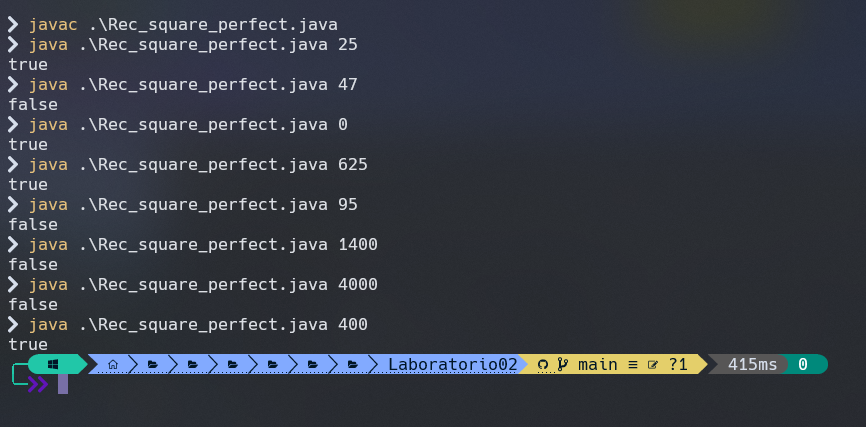
\includegraphics[width=0.9\textwidth,keepaspectratio]{img/ejec_cuadrado.png}
\end{figure}

\subsubsection{Suma de conjuntos extrema}

\begin{figure}[H]
	\centering
	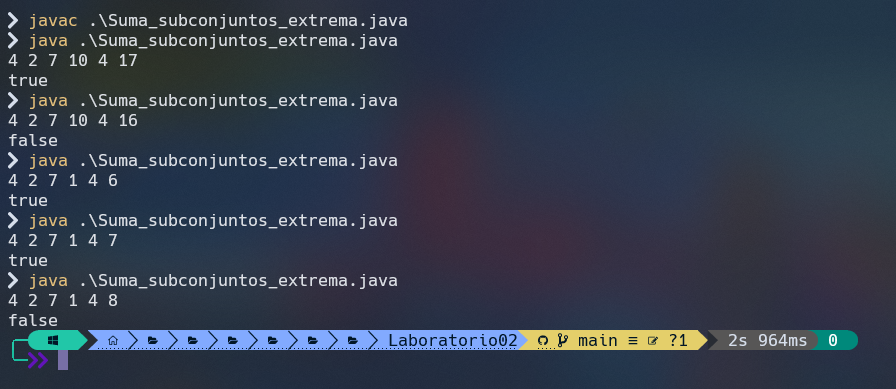
\includegraphics[width=0.9\textwidth,keepaspectratio]{img/ejec_suma.png}
\end{figure}

%%%%%%%%%%%%%%%%%%%%%%%%%%%%%%%%%%%%%%%%%%%%%%%%%%%%%%%%%%%%%%%%%%%%%%%%%%%%%%%%%%

	\subsection{Commits del trabajo}
	\begin{itemize}	
		\item Acá estan algunos de los commits mas importantes en este trabajo:
	\end{itemize}	
	
	\begin{figure}[H]
		\centering
		\includegraphics[width=0.9\textwidth,keepaspectratio]{img/Commits.png}
		%\includesvg{img/automata.svg}
		%\label{img:mot2}
		%\caption{Product backlog.}
	\end{figure}


%%%%%%%%%%%%%%%%%%%%%%%%%%%%%%%%%%%%%%%%%%%%%%%%%%%%%%%%%%%%%%%%%%%%%%%%%%%%%%%%%%
\clearpage
\subsection{Instrucciones para la ejecucion}
\begin{itemize}	
	\item Para poder compilar y ejecutar ambos ejercicios desde consola, se pueden seguir los siguientes comandos compatibles para todos los SO:

\begin{lstlisting}[language=bash, caption={Compilación de los ejercicios}, numbers=none]
javac Rec_square_perfect.java Suma_subconjuntos_extrema.java
\end{lstlisting}

\begin{lstlisting}[language=bash, caption={Ejecución de los ejercicios}, numbers=none]
java Rec_square_perfect [num]
java Suma_subconjuntos_extrema
\end{lstlisting}


\end{itemize}	


\section{Referencias}
\begin{itemize}			
	\item \url{https://dialnet.unirioja.es/servlet/articulo?codigo=4573315}
	\item \url{https://www.fdi.ucm.es/profesor/gmendez/docs/edi0910/_02-Recursion.pdf}
    \item \url{https://docs.oracle.com/javase/tutorial/}
\end{itemize}	

\end{document}